\subsection{UC-14}

\begin{figure}[H]
    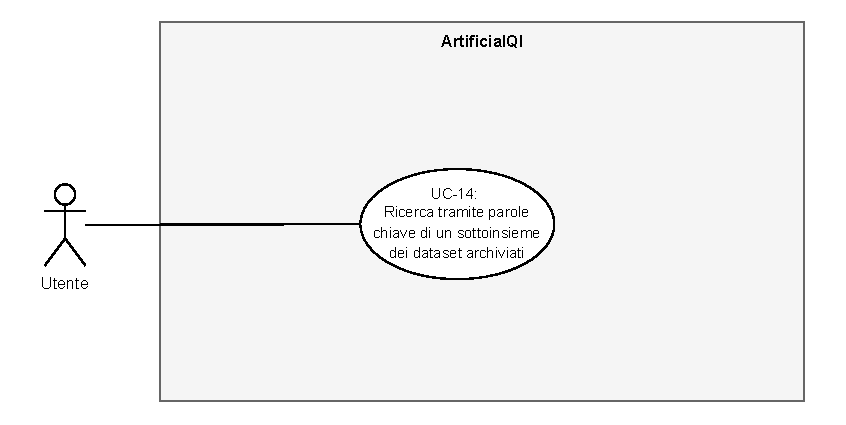
\includegraphics{Sezioni/UseCase/Immagini/UC-14.pdf}
    \caption{Diagramma UC-14.}
\end{figure}

\begin{usecase}{UC-14}{Ricerca tramite parole chiave di un sottoinsieme dei dataset archiviati}
    
    \req{\hyperref[item:RU-4]{RU-4}} 

    \pre{
        \item Il sistema è attivo e funzionante
        \item Esiste almeno un dataset archiviato
    }

    \post{
        \item Viene mostrato il sottoinsieme dei dataset archiviati risultante dall'operazione di ricerca
    }
    
    \actor{Utente}

    \subactors{}

    \trigger{L'utente deve cercare il nome di un dataset archiviato}
    
    \inc{}

    \base{}

    \scenario{
        \item L'utente specifica le parole chiave
        \item L'utente conferma l'esecuzione della ricerca
        \item Viene mostrata la lista dei dataset che contengono le parole chiave nel proprio nome
    }

    \subscenario{
        \item[1.1] \textbf{Non vengono indicate parole chiave}
        \begin{itemize}
            \item [a.] L'utente conferma l'esecuzione della ricerca
            \item [b.] Viene mostrata l'intera lista dei dataset archiviati
        \end{itemize}
        \item[3.1]\textbf{Il sottoinsieme risultante è vuoto}
        \begin{itemize}
            \item[a.] Viene notificato all'utente che la ricerca non ha prodotto risultati
        \end{itemize}
    }
\end{usecase}
